\chapter{Experiment and Result}
brief of experiment and result.
\section{Experiment}
Please tell how the experiment conducted from method.

\section{Result}
Please provide the result of experiment

\section{Aip Suprapto Munari/1164063}

\subsection{Teori}
\begin{enumerate}
\item Klasifikasi teks
	\par Klasifikasi teks atau kategorisasi teks merupakan proses yang secara otomatis menempatkan dokumen teks ke dalam suatu kategori berdasarkan isi dari teks tersebut. 
	\begin{figure}[ht]
		\centering
		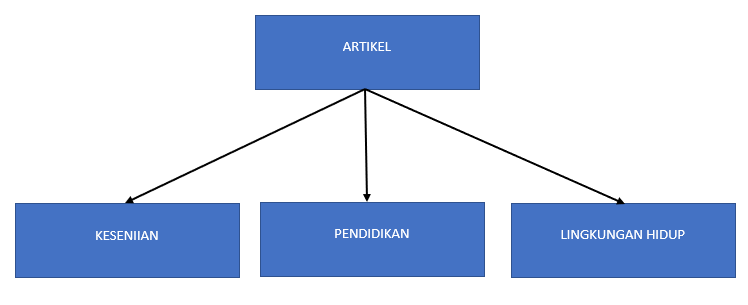
\includegraphics[scale=0.5]{figures/AIP/b1.PNG}
		\caption{Aip-Klasifikasi teks}
		\label{contoh}
	\end{figure}
	
\item Klasifikasi Bunga tidak dapat penggunakan machine learning
	\par Dikarenakan masalah dari input yang serupa namun output yang berbeda ‘noise’, yang dimaksud dengan noise adalah contoh pada output yang direkam bukan seperti perkiraan.
	\begin{figure}[ht]
		\centering
		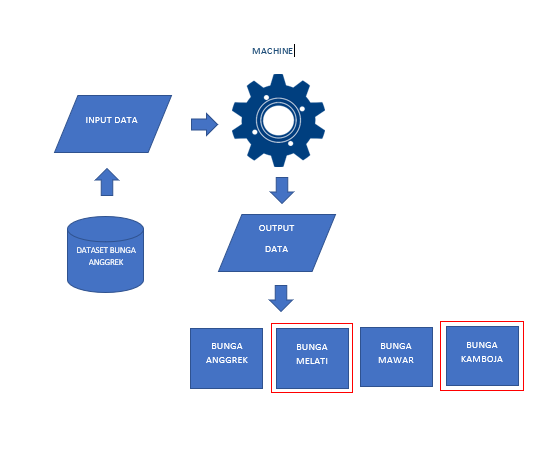
\includegraphics[scale=0.5]{figures/AIP/b2.PNG}
		\caption{Aip-Klasifikasi bunga}
		\label{contoh}
	\end{figure}

\item Teknik pembelajaran mesin pada teks YouTube
	\par Teknik Machine Learning pada YouTube memperhatikan apa saja yang menarik perhatian para penggunanya. Ketika kita sedang menonton di YouTube, pada sebelah kanan terdapat 'Up Next' yang menampilkan beberapa video serupa yang sedang ditonton. Dan ketika mengklik salah satu video dari baris tersebut, maka YouTube akan mengingatnya dan menggunakan kata yang tertera sebagai referensi.
	\begin{figure}[ht]
		\centering
		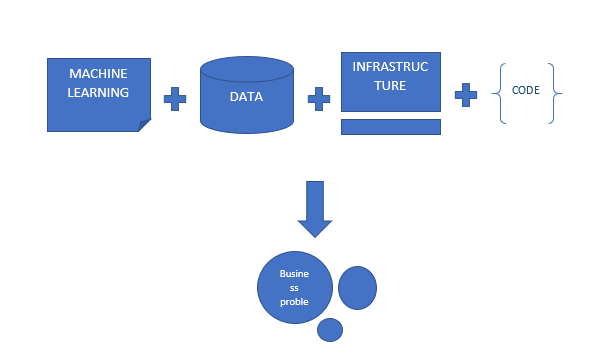
\includegraphics[scale=0.5]{figures/AIP/b3.PNG}
		\caption{Aip-Teknik YouTube}
		\label{contoh}
	\end{figure}

\item Vectorisasi Data
	\begin{itemize}
		\item Vectorisasi Data merupakan pemecahan serta pembagian data kemudian dilakukan perhitungan datanya.
	\end{itemize}
	
\item Bag of word
	\par Bag of Words adalah metode untuk mengekstraksi fitur dari dokumen teks.
	\begin{figure}[ht]
		\centering
		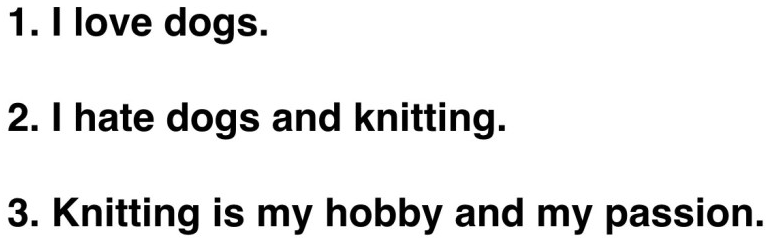
\includegraphics[scale=0.5]{figures/AIP/b4.PNG}
		\caption{Aip-Bag of Word}
		\label{contoh}
	\end{figure}
	
\item TF-IDF
	\par TF-IDF merupakan istilah beberapa frekuensi dokumen terbalik, adalah ukuran penilaian yang banyak digunakan dalam pengambilan informasi (IR) atau peringkasan. 
	\begin{figure}[ht]
		\centering
		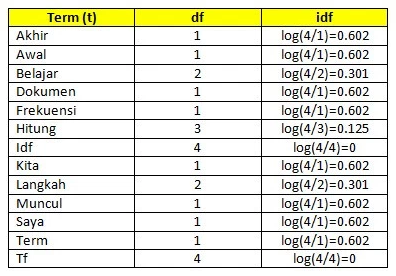
\includegraphics[scale=0.5]{figures/AIP/b5.PNG}
		\caption{Aip-TF IDF}
		\label{contoh}
	\end{figure}
\end{enumerate}

\section{BAGIAN PRAKTEK}
\section{Aip Suprapto Munari /1164063}

\subsection{Aplikasi Sederhana Menggunakan Pandas}
Disini saya akan menggunakana Dataset dari https://data.world/alexandra/generic-food-database dan akan mengambil Data Dummy sebanyak 500 records dan membuat Dataframe baru.
\begin{verbatim}
import pandas as pd
gf = pd.read_csv('D:/KULIAH/SEMESTER 6/KECERDASAN BUATAN/PRAKTEK/Python-Artificial-Intelligence-Projects-for-Beginners-master/Chapter03/generic-food.csv', sep=';')
df = pd.DataFrame(gf, columns = ['FOOD NAME', 'SCIENTIFIC NAME', 'GROUP', 'SUB GROUP'])

dummy = pd.get_dummies (df['test preparation course'])
dummy.head()
 
df = df.join(dummy)
\end{verbatim}
Maksud dari kodingan diatas yaitu :
\begin{enumerate}
\item Baris pertama impor librari pandas dengan inisiasi pd
\item Definisikan variabel gf (generic-food) untuk membaca file csv dengan pandas
\item variabel df akan menggunakan function pd dataframe untuk membuat datafarme di pandas dari file CSV yang tadi.
\item Mendefinisikan variabel dummy untuk mengubah data categorical menjadi integer. dibahwa merupakan data sebelum di Dummy. 
\begin{figure}[ht]
\centering
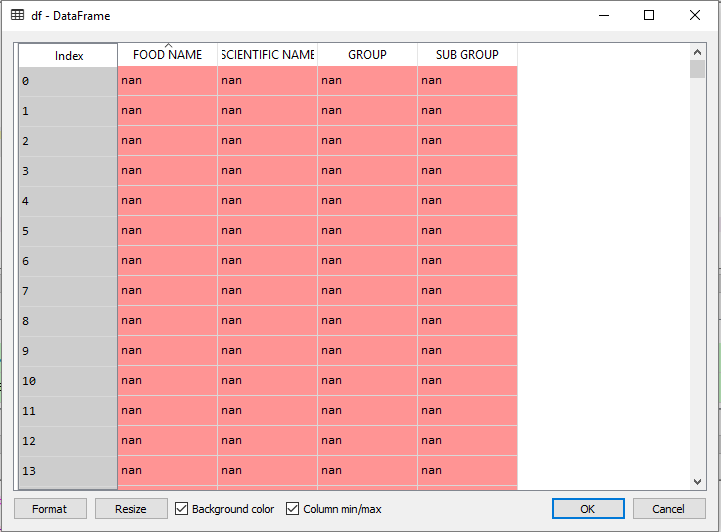
\includegraphics[scale=0.5]{figures/AIP/c2.PNG}
\caption{Dataset Original Aip}
\label{Aplikasi Pandas}
\end{figure}

\item Atribut atau kolom yang ingin di Dummy yaitu test preparation course. Dalam test memunculkan index dan nama keseluruhan kolom.
\begin{figure}[ht]
\centering
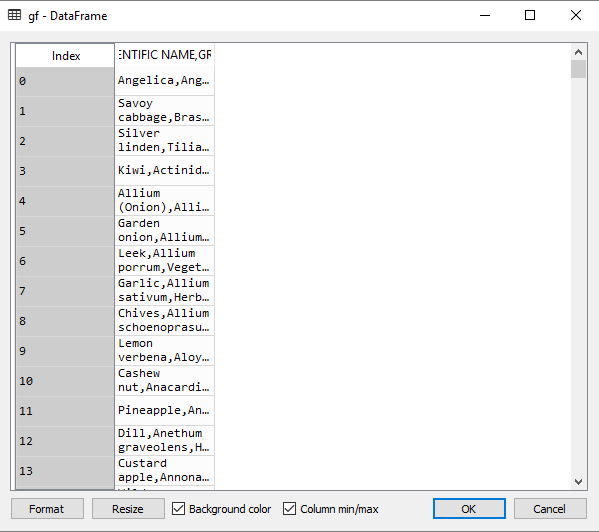
\includegraphics[scale=0.5]{figures/AIP/c3.PNG}
\caption{Dataset Dummy Aip}
\label{Aplikasi Pandas}
\end{figure}
\item kemudian df akan melakukan join dengan dataframe dummy.
\end{enumerate}

\subsection{Memecah DataFrame Menjadi 2 Dataframe}
Dari dataframe tersebut dipecah menjadi dua dataframe yaitu 450 row pertama dan 50 row sisanya
\begin{verbatim}
gf_train= gf[:450]
gf_test= gf[451:]
\end{verbatim}
\begin{enumerate}
\item gf train akan mendefinisikan dataframe untuk train dengan 450 data pertama
\item gf test mendefinisikan dataframe untuk test untuk data setelah 451. Hasilnya seperti berikut :
\end{enumerate}
\begin{figure}[ht]
\centering
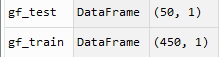
\includegraphics[scale=0.5]{figures/AIP/c4.PNG}
\caption{Split DataFrame Aip}
\label{Aplikasi Pandas}
\end{figure}

\subsection{ Vektorisasi Dan Klasifikasi Dari Data Youtube05-Shakira Dengan Decision Tree}
\begin{enumerate}
\item Ini hasil dari impor dataset
\begin{figure}[ht]
\centering
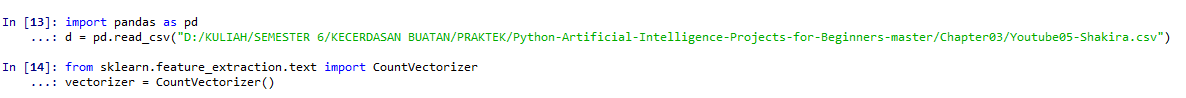
\includegraphics[scale=0.5]{figures/AIP/c7.PNG}
\caption{Dataset Youtube05-Shakira Aip}
\label{Praktek}
\end{figure}
\item Ini hasil Setelah di Klasifikasikan dengan Decision Tree
\begin{figure}[ht]
\centering
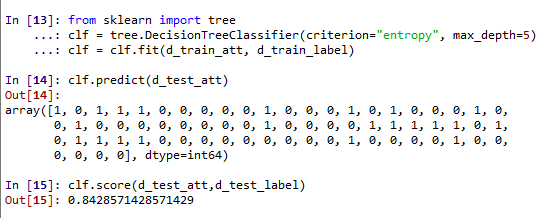
\includegraphics[scale=0.5]{figures/AIP/c6.PNG}
\caption{Dataset Youtube05-Shakira Aip}
\label{Praktek}
\end{figure}
\item Dalam in 13 impor Tree dari Sklearn. Dan mendefinisikan variabel clf untuk memanggil Decision Tree Classifier dan melakukan fit atau pengujian.
\item Dalam In 14 menggunakan prediksi untuk clf dengan function predict  untuk memprediksi test. Dan hasilnya muncul dalam bentuk array.
\item clf score memunculkan akurasi prediksi yang dilakukan terhadap clf.
\end{enumerate}

\subsection{Vektorisasi Dan Klasifikasi Dari Data Youtube05-Shakira Dengan SVM}
\begin{figure}[ht]
\centering
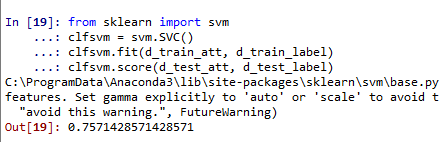
\includegraphics[scale=0.5]{figures/AIP/c8.PNG}
\caption{Dataset Youtube05-Shakira SVM Aip}
\label{Praktek}
\end{figure}
Dari Gambar diatas dapat dijelaskan bahwa :
\begin{enumerate}
\item Impor SVM dari sklearn
\item Melakukan fit dari d train att dan d train label atau disebut dengan pengujian
\item Mendefinisikan variabel clf untuk melakukan prediksi dataset Youtube05-Shakira dengan SVM. Dan akan muncul hasil prediksinya
\end{enumerate}

\subsection{Vektorisasi Dan Klasifikasi Dari Data Youtube05-Shakira Dengan Decision Tree 2}
\begin{figure}[ht]
\centering
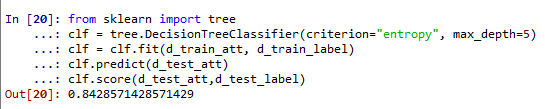
\includegraphics[scale=0.5]{figures/AIP/c9.PNG}
\caption{Dataset Youtube05-Shakira Aip}
\label{Praktek}
\end{figure}
Maksud dari codingan diatas yaitu, mengkasifikasikan Dataset Youtube05-Shakira dengan Decision Tree dengan melakukan prediksi menggunakan function test pada d test att, dan memberikan akurasi prediksi menggunakan prediksi score.

\subsection{Plotting Confusion Matrix}
Berikut adalah skripl dari plotting confusion matrix dari contoh yang ada pada bagian teori
\begin{verbatim}
import matplotlib.pyplot as plt
import itertools
def plot_confusion_matrix(cm, classes,
                          normalize=False,
                          title='Confusion matrix',
                          cmap=plt.cm.Blues):
    """
    This function prints and plots the confusion matrix.
    Normalization can be applied by setting `normalize=True`.
    """
    if normalize:
        cm = cm.astype('float') / cm.sum(axis=1)[:, np.newaxis]
        print("Normalized confusion matrix")
    else:
        print('Confusion matrix, without normalization')

    print(cm)

    plt.imshow(cm, interpolation='nearest', cmap=cmap)
    plt.title(title)
    #plt.colorbar()
    tick_marks = np.arange(len(classes))
    plt.xticks(tick_marks, classes, rotation=90)
    plt.yticks(tick_marks, classes)

    fmt = '.2f' if normalize else 'd'
    thresh = cm.max() / 2.
    #for i, j in itertools.product(range(cm.shape[0]), range(cm.shape[1])):
    #    plt.text(j, i, format(cm[i, j], fmt),
    #             horizontalalignment="center",
    #             color="white" if cm[i, j] > thresh else "black")

    plt.tight_layout()
    plt.ylabel('True label')
    plt.xlabel('Predicted label')
    

import numpy as np
np.set_printoptions(precision=2)
plt.figure(figsize=(60,60), dpi=300)
plot_confusion_matrix(cm, classes=clf, normalize=True)
plt.show()
\end{verbatim}
Hasilnya adalah sebagai berikut :
\begin{figure}[ht]
\centering
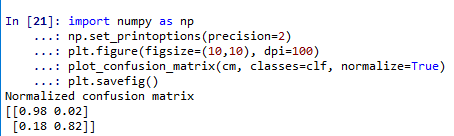
\includegraphics[scale=0.5]{figures/AIP/c10.PNG}
\caption{Confusion Matrix Aip}
\label{Praktek}
\end{figure}
Dari gambar dapat dijelaskan bahwa data array merupakan data asli dan data prediksi yang dilakukan dengan Random Forest. Dengan melakukan normalisasi data confusion matrix.

\subsection{ Menjalankan Program Cross Validation}
\begin{figure}[ht]
\centering
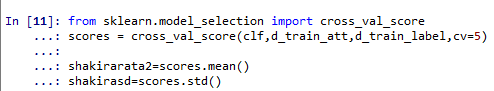
\includegraphics[scale=0.5]{figures/AIP/c5.PNG}
\caption{Cross Validation Aip}
\label{Aplikasi Pandas}
\end{figure}
Gambar diatas akan dijelaskan seperti berikut :
\begin{enumerate}
\item Dari sklearn mengimpor Cross Validation
\item Variabel scores akan melakukan cross validation pada variabel clf, d train att , dan d train label
\item Variabel shakirarata2 akan menghitung nilai rata rata dari variabel scores tadi menggunakan function mean
\item shakirasd Menghitung standar deviasi dari data yang diberikan. Hasilnya seperti berikut :
\end{enumerate}
\begin{figure}[ht]
\centering
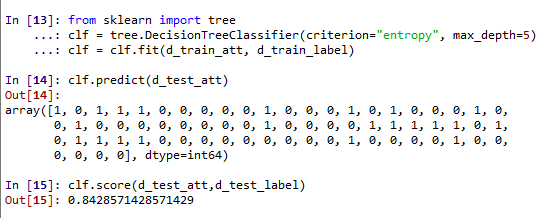
\includegraphics[scale=0.5]{figures/AIP/c6.PNG}
\caption{Hasil Cross Validation Aip}
\label{Cross Validation}
\end{figure}

\subsection{Program Pengamatan Komponen Informasi}
\begin{figure}[ht]
\centering
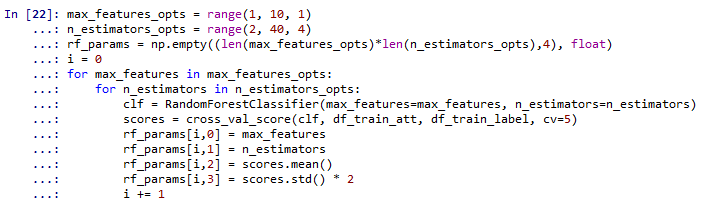
\includegraphics[scale=0.5]{figures/AIP/c11.PNG}
\caption{Program Komponen Informas Aip}
\label{Praktek}
\end{figure}
Dari gambar diatas dapat dijelaskan bahwa :
\begin{enumerate}
\item Max featuresnya dari range 1 sampai 10
\item n estimators dengan range 20 sampai 40
\item Variabel rf params berisikan function np empty dimana akan membuat array baru berisikan tipe yang didefinisikan dengan random value
\item Mendefinisika i dimulai dari angka 0 dimana max features dan n estimators menggunakan klasifikasi randomforestclassifier menggunakan data prediksi
\item Mendefinisikan rfparams untuk max features , n estimators, nilai rata dan std
\end{enumerate}

\section{Penanganan Error}
AIP SUPRAPTO MUNARI 1164063
\subsection{Error Index}
\begin{enumerate}
	\item
Berikut ini merupakan eror yang didapatkan saat menjalankan program diatas
\begin{figure}[ht]
\centering
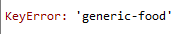
\includegraphics[scale=0.5]{figures/AIP/errorc1.PNG}
\caption{Error Key Aip }
\label{Error}
\end{figure}
\item
Pada gambar diatas kode erornya adalah KeyEror. Eror ini terjadi karena keyword yang dimasukan tidak ada.
\item
Solusi yang bisa dilakukan untuk mengatasi eror tersebut adalah sebagai berikut : 
\end{enumerate}
\begin{itemize}
\item
\begin{figure}[ht]
\centering
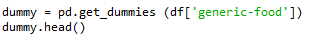
\includegraphics[scale=0.5]{figures/AIP/errorc2.PNG}
\caption{Error Key Aip}
\label{Error}
\end{figure}
Pada gambar diatas Dataset Generic-Food tidak terdapat atribut COLOR, maka dari itu kita harus merubahnya dengan atribut yang terdapat di dataset tersebut. Mari kita gunakan atribut SCIENTIFIC NAME. Ubah skrip menjadi seperti berikut
\item
\begin{figure}[ht]
\centering
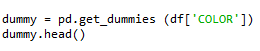
\includegraphics[scale=0.5]{figures/AIP/errorc3.PNG}
\caption{Error Key Aip}
\label{Error}
\end{figure}
\item Maka ketika di run akan muncul data dummy nya seperti berikut
\begin{figure}[ht]
\centering
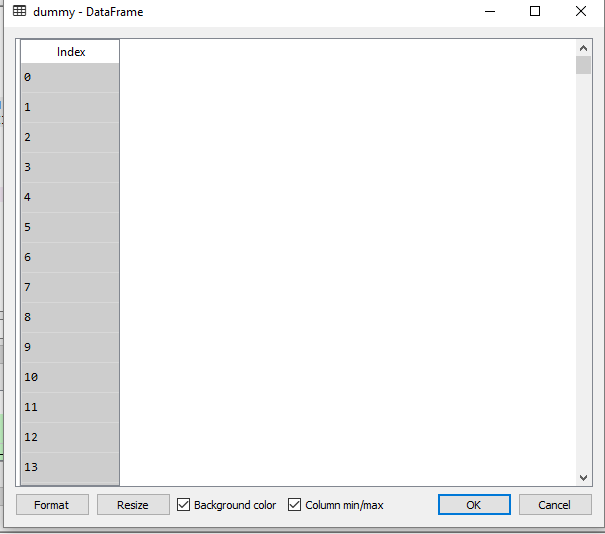
\includegraphics[scale=0.5]{figures/AIP/errorc4.PNG}
\caption{Error Key Aip}
\label{Error}
\end{figure}
\end{itemize}




\section{Andi Muhammad Aslam/1164064}

\subsection{Teori}
\begin{enumerate}
\item Klasifikasi teks
	\par Klasifikasi merupakan kata serapan dari bahasa Belanda, classificatie, yang sendirinya berasal dari bahasa Prancis classification. Istilah ini menunjuk kepada sebuah metode untuk menyusun data secara sistematis atau menurut beberapa aturan atau kaidah yang telah ditetapkan.
	Di dalam KBBI, klasifikasi adalah penyusunan bersistem dalam kelompok atau golongan menurut kaidah atau standar yang ditetapkan. Secara harafiah bisa pula dikatakan bahwa klasifikasi adalah pembagian sesuatu menurut kelas-kelas. Menurut Ilmu Pengetahuan, Klasifikasi adalah Proses pengelompokkan benda berdasarkan ciri-ciri persamaan dan perbedaan.
	\begin{figure}[ht]
		\centering
		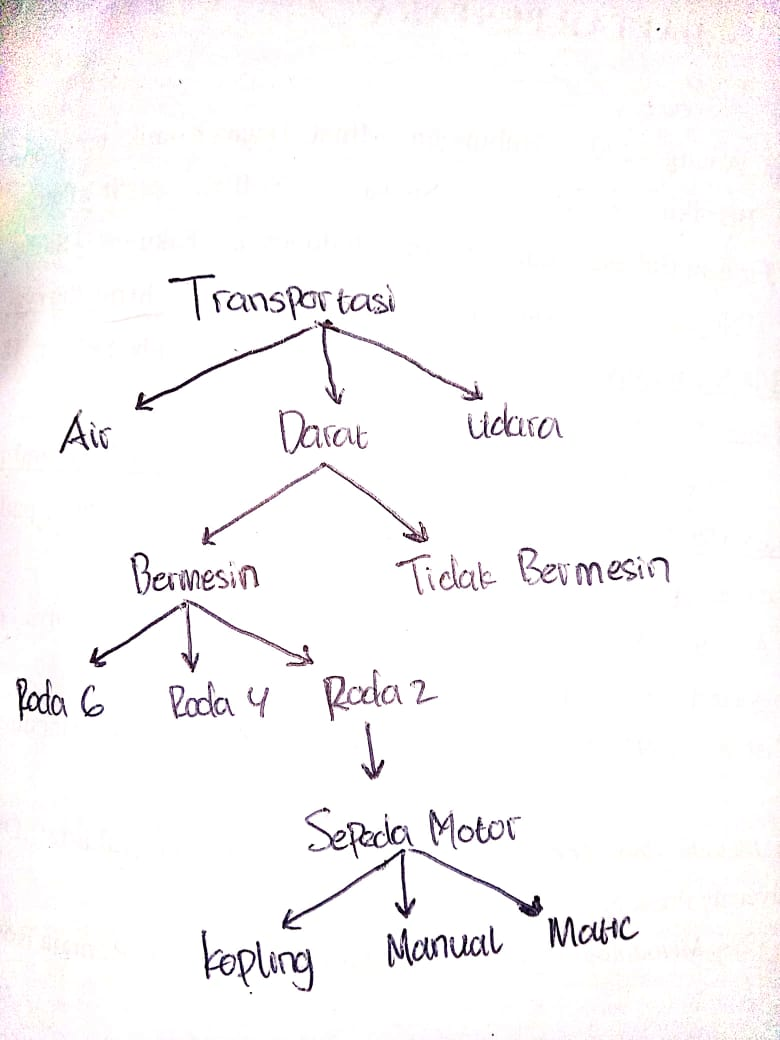
\includegraphics[scale=0.5]{figures/andi/4-1.jpeg}
		\caption{Klasifikasi teks}
		\label{Contoh Ilustrasi}
	\end{figure}
	
\item Klasifikasi Bunga tidak bisa menggunakan machine learning
	\par Machine Learning tidak dapat mengklasifikasikan bunga, Karena data yang diberikan pada 
mesin itu akan di algoritmakan untuk mencari sesuatu yang menarik dalam data yang kita 
berikan, hingga akhirnya sistem AI akan membangun pengetahuan berdasarkan data tersebut.
Dengan kata lain, pembelajaran mesin data beradaptasi terhadap suatu masalah dengan mempelajari pola-pola yang ditemukan dalam data
Sebagai contoh data pada spesies bunga dari genus Iris dengan melihat ukuran sepal (kelopak) dan petalnya(mahkota) pada algoritma data bunga tersebut akan melatih proses pembelajaran pada mesin dalam menganalisa spesies bunga Iris. Dan algoritma pembelajaran mesin akan mempelajari karakteristik dari masing-masing spesies bunga Iris berdasarkan ukuran sepal dan petal yang diberikan.
	\begin{figure}[ht]
		\centering
		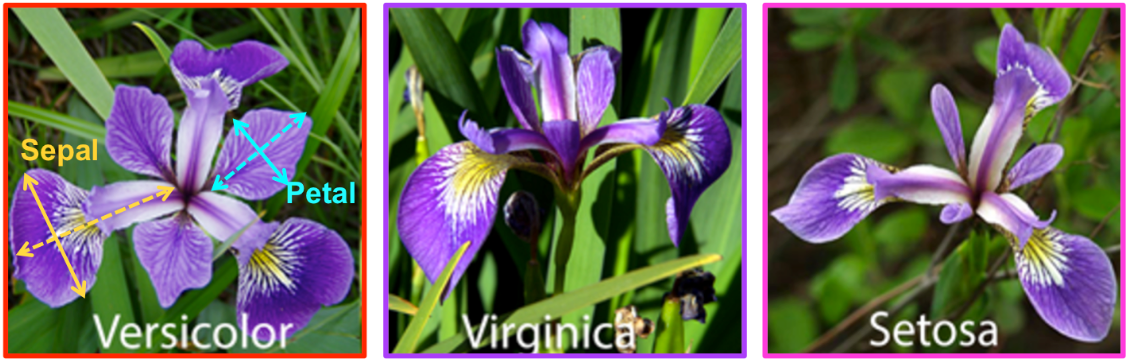
\includegraphics[scale=0.5]{figures/andi/4-2.png}
		\caption{Klasifikasi bunga}
		\label{Contoh Ilustrasi}
	\end{figure}

\item Youtube memungkinkan agar mendapatkan video yang direkomendasikan, karena Machine Learning pada Youtube pasti akan melibatkan data yang sering di lihat oleh penggunanya.
Youtube juga akan memberitahukan si pengguna apabila ada video baru yang telah di upload pada chanel yang direkomendasikan untuk si pengguna. Dan apabila menonton video pada youtube maka youtube dapat mengingat dan menggunakan kata tersebut sebagai referensi.
	\begin{figure}[ht]
		\centering
		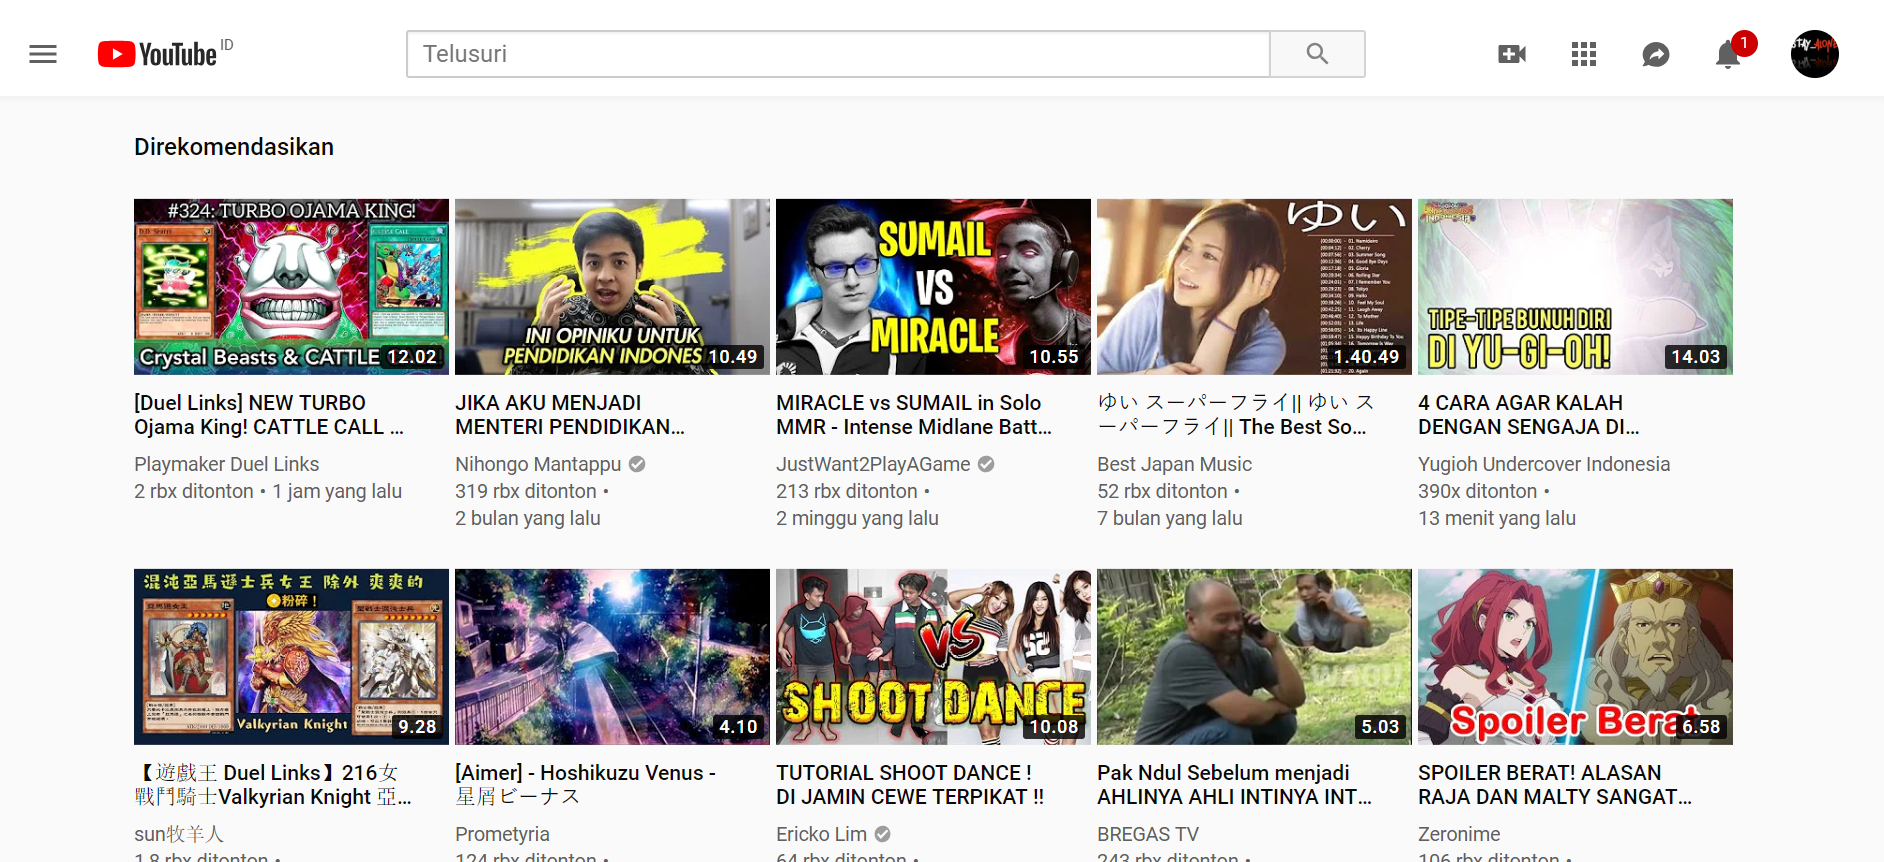
\includegraphics[scale=0.5]{figures/andi/4-3.PNG}
		\caption{Teknik YouTube}
		\label{Contoh Ilustrasi}
	\end{figure}

\item Vectorisasi Data
	\begin{itemize}
		\item proses vektorisasi ini menghasilkan suatu wujud peta yang menggambarkan keadaan permukaan bumi atau bentang alam. Sifat data yang geometris menunjukkan ukuran dimensi yang sesungguhnya.
	\end{itemize}
	
\item Bag of word
	\par Bag of word merupakan konsep yang diambil dari analisis, kemudian merepresentasikan dokumen berupa kumpulan informasi penting tanpa mengurutkan setiap katanya.
	\begin{figure}[ht]
		\centering
		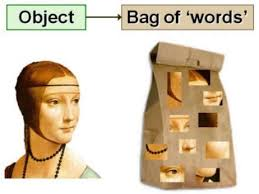
\includegraphics[scale=0.5]{figures/andi/4-5.jpg}
		\caption{Bag of Word}
		\label{Contoh Ilustrasi}
	\end{figure}
	
\item TF-IDF
	\par TF-IDF dimaksudkan untuk mencerminkan seberapa relevan suatu istilah dalam dokumen yang diberikan. Intuisi di baliknya adalah bahwa jika sebuah kata muncul beberapa kali dalam sebuah dokumen, kita harus meningkatkan relevansinya karena itu harus lebih bermakna daripada kata-kata lain yang muncul lebih sedikit kali (TF). Pada saat yang sama, jika sebuah kata muncul berkali-kali dalam suatu dokumen tetapi juga di sepanjang banyak dokumen lain, mungkin itu karena kata ini hanya kata yang sering; bukan karena itu relevan atau bermakna (IDF).
	\begin{figure}[ht]
		\centering
		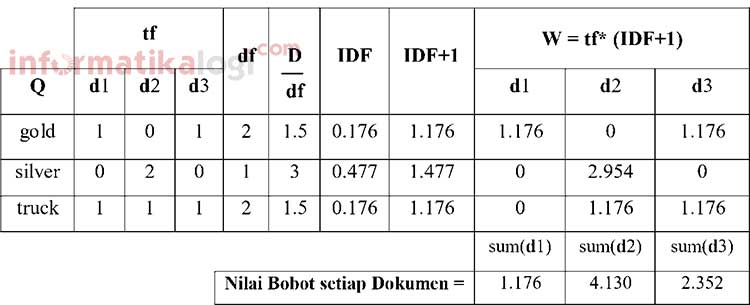
\includegraphics[scale=0.5]{figures/andi/4-6.jpg}
		\caption{TF-IDF}
		\label{Contoh Ilustrasi}
	\end{figure}
\end{enumerate}







\section{Andi Muhammad Aslam/1164064}

\subsection{Praktek Program}
\begin{enumerate}
\item Pada penjelasan kali ini saya akan membuat data dummy dengan menggunakan format csv, data di ambil dari web UCI Machine Learning
\par Repository dengan nama file Youtube02-KatyPerry.csv  
\begin{figure}[ht]
	\centerline{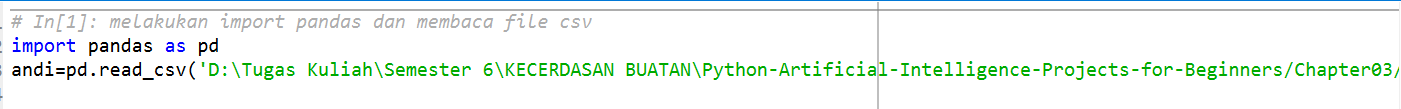
\includegraphics[width=1\textwidth]{figures/andi/G1.PNG}}
	\caption{Data Dummy 500 Data}
	\label{Contoh Ilustrasi}
\end{figure}

\subitem Penjelasan pada gambar G1 yaitu mengimport librari pandas dimana kita mengaliaskan praktek sebagai pandas. Pandas berguna untuk mengelola  dataframe = matrix = tabel kemudian memanggil nama alias untuk membaca format csvnya.
\item Dari dataframe yang sudah ada sebelumnya kita akan membagi menjadi 2 yaitu 450 row pertama dan 50 row 
\par Dapat dilihat pada gambar \ref{G2}
\begin{figure}[ht]
	\centerline{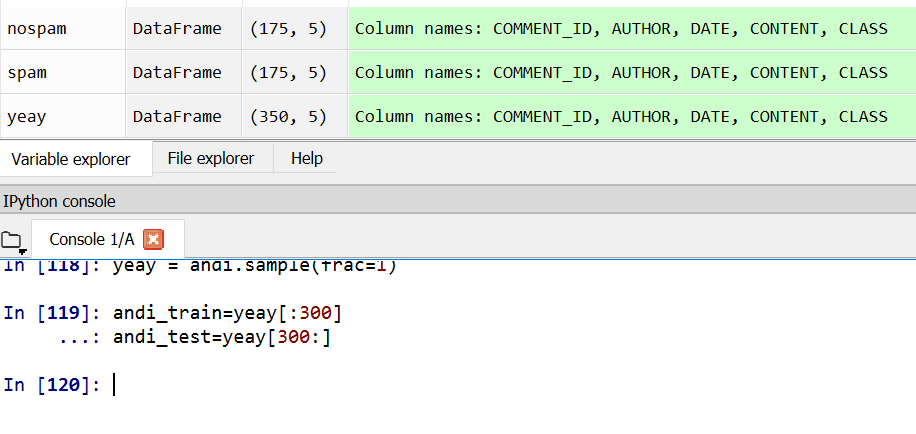
\includegraphics[width=1\textwidth]{figures/andi/G2.PNG}}
	\caption{Membagi 2 Dataframe}
	\label{Contoh Ilustrasi}
\end{figure}

\subitem Penjelasan pada gambar G2 yaitu baris pertama dimana d\_train untuk membagi data training sebanyak 450 row dan pada 
\par baris kedua dimana d\_test untuk data sisa atau data yang baru sebanyak 50 row.
\item Melakukan Vektorisasi dan Klasifikasi Data pada data KetyPerry pada gambar G3  merupakan dataframe keseluruhan dari file csv yang sudah dimasukkan dengan jumlah 448 baris dan 5 kolom. nospam merupakan dataframe yang isinya hanya data yang bukan termasuk spam dengan inisial angka 0. Sedangkan spam merupakan dataframe yang isinya hanya data spam dengan inisial angka 1.
\begin{figure}[ht]
	\centerline{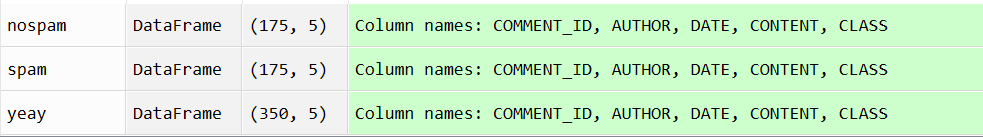
\includegraphics[width=1\textwidth]{figures/andi/G3.PNG}}
	\caption{Vektorisasi dan Klasifikasi Data}
	\label{Contoh Ilustrasi}
\end{figure}

\subitem  Pada gambar G3 merupakan hasil output content dimana terdapat 448 baris/data yang mempunyai 1602 kata-kata yang digunakan pada komentar yang ada di content tersebut.
\begin{figure}[ht]
	\centerline{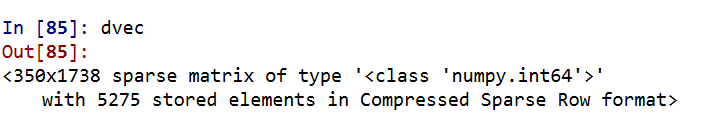
\includegraphics[width=1\textwidth]{figures/andi/G4.PNG}}
	\caption{Data Content}
	\label{Contoh Ilustrasi}
\end{figure}

\subitem Pada gambar G4 maksud dari outputannya merupakan dataframe kata-kata tadi yang berjumlah 1602 kata orang 
 yang komen pada data KetyPerry.
\begin{figure}[ht]
	\centerline{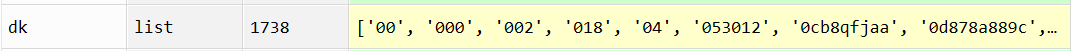
\includegraphics[width=1\textwidth]{figures/andi/G5.PNG}}
	\caption{DataFrame Kata-kata Pada Content}
	\label{Contoh Ilustrasi}
\end{figure}

\item Mengklasifikasikan dari data vektorisasi dengan menggunakan klasifikasi svm(support vektorisasi machine) dapat dilihat pada  gambar G6.
\begin{figure}[ht]
	\centerline{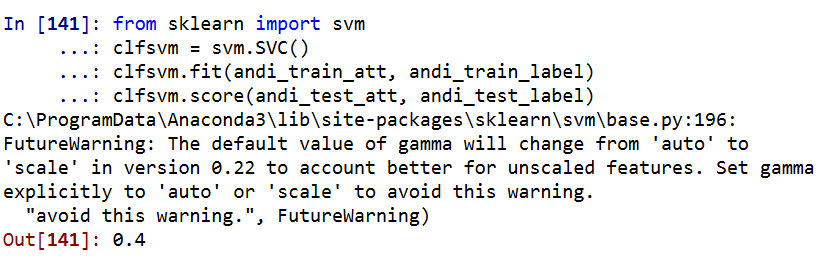
\includegraphics[width=1\textwidth]{figures/andi/G6.PNG}}
	\caption{Klasifikasi SVM Dari Data Vektorisasi}
	\label{Contoh Ilustrasi}
\end{figure}

\subitem Jadi pada gambar G6 merupakan hasil dari memprediksi data score vektorisasi dengan svm menggunakan metode fit dimana digunakan untuk data training atau data pelatihannya.
\item Mengklasifikasikan dari data vektorisasi dengan menggunakan klasifikasi Decision Tree dapat dilihat pada gambar G7.
\begin{figure}[ht]
	\centerline{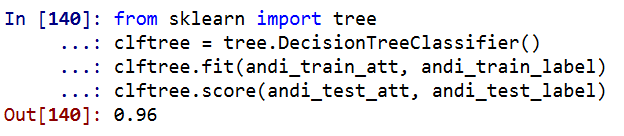
\includegraphics[width=1\textwidth]{figures/andi/G7.PNG}}
	\caption{Klasifikasi Decision Tree Dari Data Vektorisasi}
	\label{Contoh Ilustrasi}
\end{figure}

\subitem Jadi pada gambar G7 merupakan hasil dari memprediksi data score vektorisasi dengan Decision Tree menggunakan metode fit dimana digunakan untuk data training atau data pelatihannya saja.
\item Mengeplot confusion matrix menggunakan matplotlib dapat dilihat pada gambar G8.
\begin{figure}[ht]
	\centerline{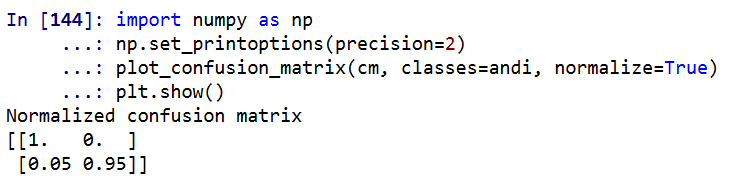
\includegraphics[width=1\textwidth]{figures/andi/G8.PNG}}
	\caption{Plot Confusion Matrix Menggunakan Matplotlib}
	\label{Contoh Ilustrasi}
\end{figure}

\subitem Pada gambar G8 sebelumnya kita harus mengimport matplotlibnya terlebih dahulu setelah itu di sini saya 
 menggunakan numpy untuk mengeluarkan hasil plot confusion matrix pada matplolibnya nantinya akan keluar normalisasi dari  confusion matrix berupa data baris dan kolom. 
\item Menjalankan program cross validation pada data vektorisasi dapat dilihat pada gambar G9.
\begin{figure}[ht]
	\centerline{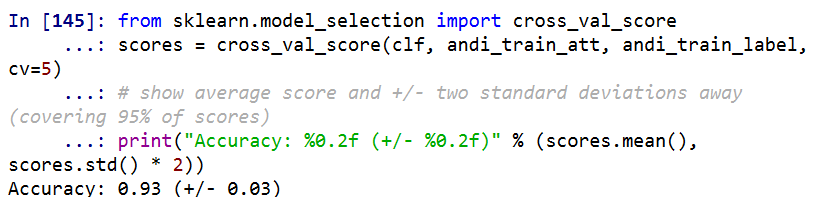
\includegraphics[width=1\textwidth]{figures/andi/G9.PNG}}
	\caption{Program Cross Validation Pada Data Vektorisasi}
	\label{Contoh Ilustrasi}
\end{figure}

\subitem Pada gambar G9 yang pertama yaitu memunculkan akurasi cross validation dari random forest pada data yang sudah divektorisasi, yang kedua yaitu memunculkan akurasi cross validation dari decision tree pada data yang sudah divektorisasi, dan yang ketiga yaitu memunculkan akurasi cross validation dari svm pada data yang sudah divektorisasi.
\item Membuat program pengamatan komponen informasi pada data yang sudah divektorisasi dapat dilihat pada gambar G10
\begin{figure}[ht]
	\centerline{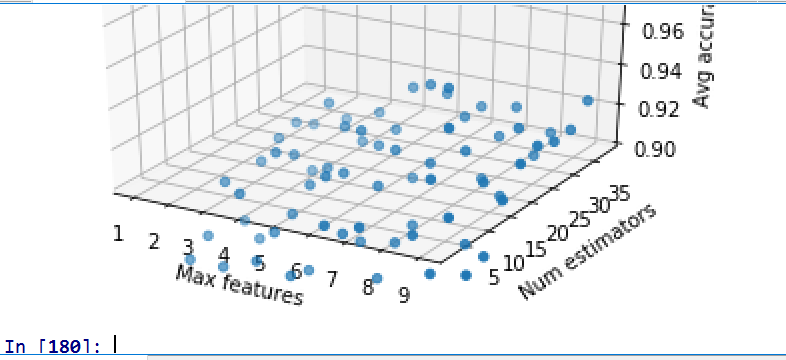
\includegraphics[width=1\textwidth]{figures/andi/G10.PNG}}
	\caption{Program Pengamatan Komponen Informasi}
	\label{Contoh Ilustrasi}
\end{figure}

\subitem Pada gambar G10  merupakan hasil outputan yang mana max features di sana terdapat 9 data dari 10 yang sudah kita masukkan ke dalam codingan sebelumnya dan penomoran estimatornya merupakan data per 5 dari angka 40 sedangkan rata-rata akurasinya kita tuliskan datanya mulai dari 0.9 sampai dengan 1. Titik-titik yang didalam tersebut merupakan data vektorisasi dari pengamatan komponen informasinya.
\end{enumerate}

\subsection{Penanganan Eror}
\begin{enumerate}
\item Pada gambar G11 merupakan ScreeShootan dari data yang eror.
\begin{figure}[ht]
	\centerline{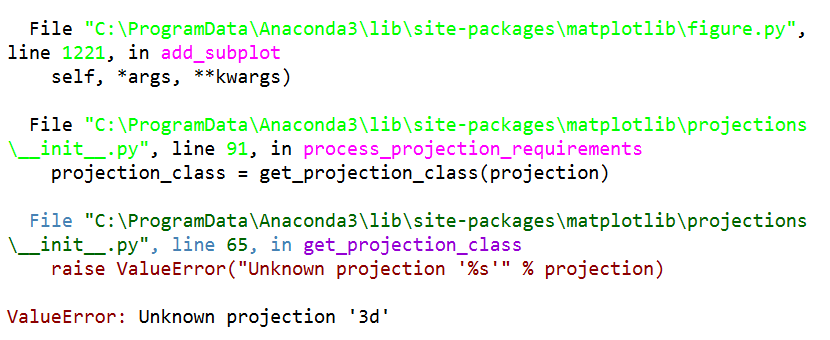
\includegraphics[width=1\textwidth]{figures/andi/G11.PNG}}
	\caption{Eror matplotlib.pyplot}
	\label{Contoh Ilustrasi}
\end{figure}

\item 
\begin{verbatim}
 matplotlib.pyplot
Traceback (most recent call last):

  File "<ipython-input-151-8094433808cc>", line 6, in <module>
    ax = fig.gca(projection='3d')

  File "C:\ProgramData\Anaconda3\lib\site-packages\matplotlib\figure.py", line 1817, in gca
    return self.add_subplot(1, 1, 1, **kwargs)

  File "C:\ProgramData\Anaconda3\lib\site-packages\matplotlib\figure.py", line 1221, in add_subplot
    self, *args, **kwargs)

  File "C:\ProgramData\Anaconda3\lib\site-packages\matplotlib\projections\__init__.py", line 91, in process_projection_requirements
    projection_class = get_projection_class(projection)

  File "C:\ProgramData\Anaconda3\lib\site-packages\matplotlib\projections\__init__.py", line 65, in get_projection_class
    raise ValueError("Unknown projection '%s'" % projection)

ValueError: Unknown projection '3d'

<Figure size 432x288 with 0 Axes>
\end{verbatim}

\item Solusi eror tersebut dengan menambahkan  menambahkan codingan tersebut seperti berikut.
\begin{verbatim}
from mpl_toolkits.mplot3d import Axes3D
from matplotlib import cm
fig = plt.figure()
fig.clf()
\end{verbatim}
\end{enumerate}

